\documentclass[11pt,a4paper]{letter}
\usepackage[top=0.50in, bottom=0.5in, left=1.1in, right=1.1in]{geometry}
\usepackage{graphicx}

%\signature{}

\usepackage{Sweave}
\begin{document}

\begin{letter}{}

\includegraphics[width=0.3\textwidth]{logo_uah.png}

\opening{Dear Dr. Wake:}

\noindent Please consider our paper, entitled `Phylogenetic estimates of species-level phenology improve ecological forecasting' as a Letter in \emph{Nature Climate Change}. Our research addresses the critical challenge of accurately predicting the impacts of climate change on plant phenology---with consequences for key ecosystem services---and highlights the importance of incorporating both species variability and phylogenetic information in forecasts.
\vspace{1.5ex}\\
Comments from three reviewers have greatly improved this manuscript and led us to present new validation and sensitivity analyses, which show that our findings are robust. Specifically, we have reanalysed our data using an alternative metric for chilling and have devised a new (leave-one-clade-out) cross-validation scheme for Bayesian Hierarchical models phylogenetic or non-phylogenetic. New results reinforce the findings from our original submission showing that, for our dataset, including phylogenetic relationships in the model improves ecological forecasting. In addition we provide a more thorough description of our data and methods and discuss in more depth the implications of our research. 
\vspace{1.5ex}\\
Reviewer 1 suggested increasing the geographic coverage of our dataset given that it only includes Northern Hemisphere temperate tree species. Unfortunately, doing so would be unfeasible because existing experimental data on phenological responses to cues are strongly biased geographically. We were aware of these limitations, which at least partly, motivated us for developing the phylogenetic model we present here. Until further experiments on extra-temperate species are conducted, quantifying uncertainty with Bayesian methods, and leveraging information on evolutionary relationships (which covary with biogeography) arise as an promising venue to generate robust predictions, even when departing from unbalanced data.
%IMC- this paragraph likely needs strong revision.
\vspace{1.5ex}\\
We have addressed all reviewer concerns including edits,  corrections to the main text and the addition of 5 figures and 3 tables to the Supporting Information. We feel the new submission is much improved and detail our changes in the response letter to reviewers (note that reviewer comments are in \emph{italics}, while our responses are in regular text).  This manuscript is not under consideration elsewhere.  We hope that you will find it suitable for publication in \emph{Nature Climate Change}, and look forward to hearing from you.


\vspace{0.25ex}\\
\vspace{1.5ex}\\


\vspace{1.5ex}\\
\noindent Sincerely,\\
\vspace{1.5ex}\\
 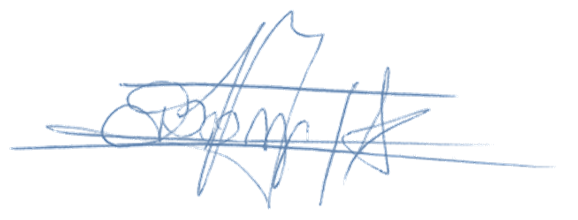
\includegraphics[width=0.2\textwidth]{Signature_IMC.png} \\
 \vspace{1.5ex}\\
\noindent Ignacio Morales-Castilla


\end{letter}
\end{document}
